\section*{Exercice 174 -- Géométrie}
% Banque PT SIA 2013 CLever

\setcounter{exo}{0}
On s'intéresse à un véhicule triporteur permettant de s'incliner en virage.
\begin{center}
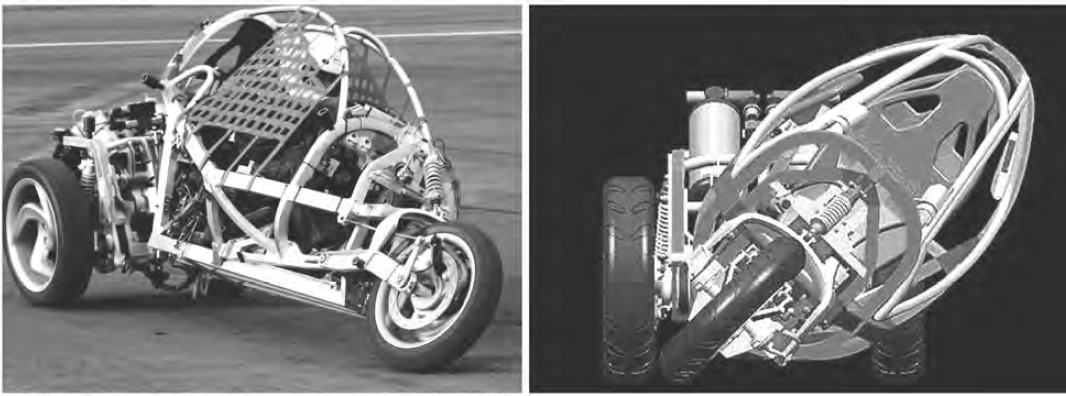
\includegraphics[width=\linewidth]{043_01}
\end{center}

 Le schéma cinématique du système de transformation de mouvement est précisé sur la figure suivante. On considère le triangle $OA_1A_2$ \textbf{(0)} comme étant le bâti. La course des vérins est de $\SI{200}{mm}$. L'ensemble \textbf{(1)} désigne l'habitacle du véhicule.


\begin{center}
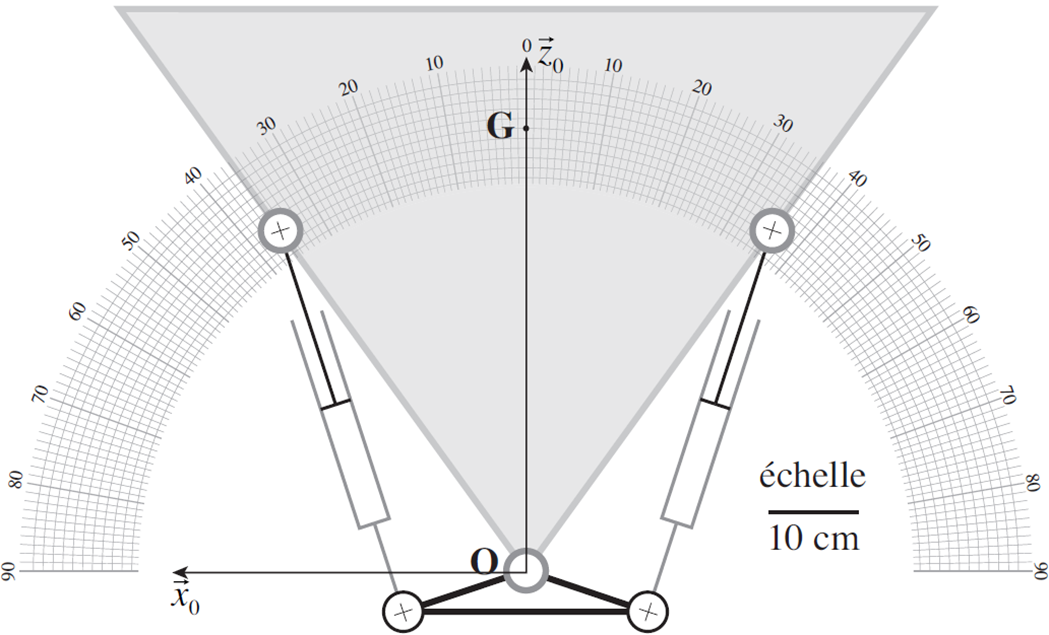
\includegraphics[width=\linewidth]{043_02}
\end{center}
 
L'habitacle doit pouvoir se dépalcer de de \SI{-45}{\degres} à \SI{+45}{\degres}. 
\subparagraph{}\textit{Déterminer la course des vérins.}